
\section{Lịch sử  các hệ điều hành}
\label{sec:31}

Máy tính trong những năm $1940$ và $1950$ rất không mềm dẻo và hiệu quả. Chúng chiếm hết
cả căn phòng, và việc thực hiện chương trình yêu cầu chuẩn bị nhiều thứ: lắp các băng từ,
đặt các bìa đục lỗ vào ổ đọc, bố trí các chuyển mạch,... Việc thực hiện chương trình (ở
đây ta gọi là \textbf{công việc} (job)) được xử lý như một hoạt động riêng biệt, và máy đã
phải đã được chuẩn bị sẵn sàng từ trước để thực hiện chương trình này.  Khi chương trình
thực hiện xong, nếu ta muốn thực hiện tiếp chương trình khác thì ta lại phải lưu trữ trước
mọi băng, thẻ đục lỗ,... Khi có nhiều người muốn chia sẻ một máy, họ phải đăng ký trước
thời gian dùng máy. Trong khoảng thời gian được cấp phép, máy hoàn toàn thuộc quyền điều
khiển của người dùng. Phiên làm việc bao gồm cài đặt chương trình (mất rất nhiều thời
gian) và chạy chương trình (trong khoảng thời gian rất ngắn). Mọi thứ luôn phải làm vội
vàng vì luôn có người đang kiên nhẫn chờ để dành máy.

Trong môi trường như vậy, các hệ điều hành ban đầu chỉ nhằm đơn giản hoá việc cài đặt
chương trình và hợp lý hoá việc chuyển đổi giữa các công việc. Những cải tiến đầu tiên là
tách riêng người sử dụng và thiết bị nhằm tránh việc có quá nhiều người ra vào phòng máy
tính. Với mục đích này, các phòng máy luôn có người trực máy. Khi người dùng muốn thực
hiện một chương trình, anh ta phải gửi chương trình, dữ liệu cần chạy, và các chỉ dẫn cụ
thể về chương trình cho người trực máy, và đợi để nhận lại kết quả chạy. Về phía người
trực máy, anh ta phải bật máy, đưa các thông tin này vào thiết bị lưu trữ khối của máy nơi
một chương trình được gọi là hệ điều hành có thể đọc và thực hiện chúng. Đây là bắt đầu
của \textbf{xử lý theo lô}--các công việc cần thực hiện được tập hợp lại và thực hiện mà
không cần tương tác với người sử dụng.


Trong các hệ thống xử lý theo lô, các công việc đợi thực hiện nằm trong một thiết bị lưu
trữ khối. Thiết bị này được gọi là \textbf{hàng đợi công việc} (job queue) (Hình
\ref{fig:fig3.1}). Một \textbf{hàng đợi} là một tập các đối tượng (trong trường hợp này là
các công việc) được tổ chức theo kiểu \textbf{vào trước, ra trước} (gọi tắt là FIFO). Có
nghĩa rằng, các đối tượng được lấy ra khỏi hàng đợi theo thứ tự chúng được đưa vào. Trên
thực tế, hầu hết các hàng đợi không tổ chức chặt chẽ theo cấu trúc FIFO mà xem xét theo độ
ưu tiên của từng đối tượng. Các hệ điều hành nói chung đều cho phép xem xét các công việc
theo độ ưu tiên. Bởi vậy, một công việc nằm trong hàng đợi dù sắp đến lượt vẫn có thể bị
đẩy về sau bởi một công việc khác có độ ưu tiên cao hơn.

\begin{figure}[bt]
\centering
    \scalebox{0.35}{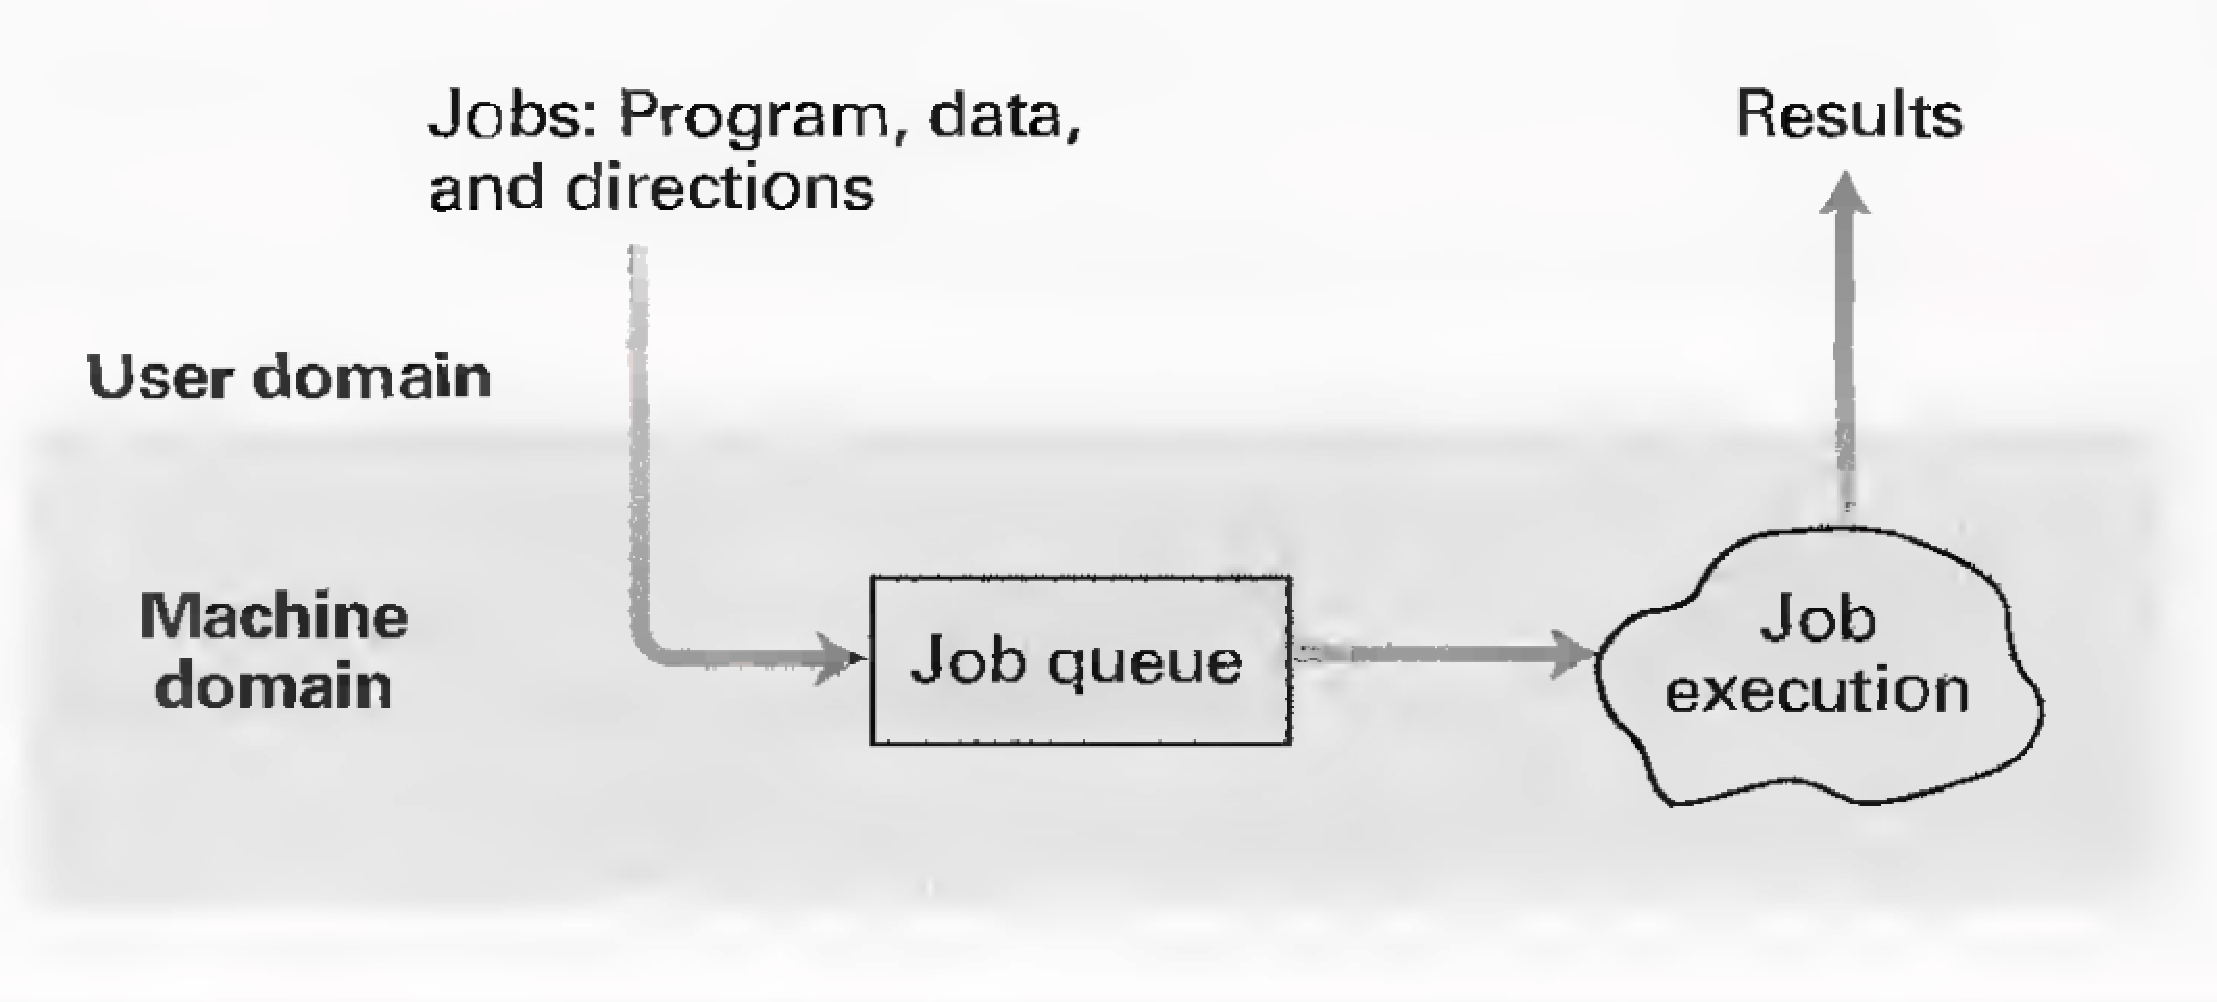
\includegraphics{ch4/fig31.pdf}}
\caption{Xử lý theo lô}
  \label{fig:fig3.1}
\end{figure}

Trong các hệ thống xử lý theo lô trước đây, mỗi công việc đi kèm với bởi một tập các chỉ
thị giải thích các bước yêu cầu người trực máy chuẩn bị theo đặc thù của công việc đó. Các
chỉ thị này được mã hoá, dùng một hệ thống gọi là ngôn ngữ điều khiển công việc (JCL). Tập
chỉ thị này được lưu trữ cùng với công việc trong hàng đợi công việc. Khi một công việc
được chọn để thực hiện, hệ điều hành in các chỉ thị này ra máy in để người trực máy tính
có thể đọc và làm theo. Ngày nay, ta vẫn thấy cách giao tiếp này, ví dụ như các báo lỗi
của hệ điều hành: ``no dial tone'', ``ổ đĩa không truy cập được'' hay ``máy in không trả
lời''.

Một trở ngại trong việc sử dụng người trực máy làm trung gian là người dùng phải gửi công
việc cho người trực máy, và do đó họ không thể tương tác được với công việc của họ. Cách
tiếp cận này có thể phù hợp với một số kiểu ứng dụng, ví dụ như xử lý bảng lương ở đó tất
cả mọi dữ liệu và cách xử lý đã được xác định trước. Tuy nhiên, trong nhiều trường hợp
cách này là không chấp nhận được, ví dụ như trong hệ thống đặt vé ở đó việc đặt và huỷ vé
phải được báo cáo ngay khi chúng xuất hiện, trong hệ thống xử lý văn bản ở đó tài liệu
được viết và viết lại liên tục, hay trong các trò chơi máy tính ở đó người dùng luôn phải
tương tác với máy.

Để thích nghi với các nhu cầu này, người ta đã phát triển các hệ điều hành mới cho phép
các chương trình thực hiện giao tiếp với người sử dụng qua trạm cuối ở xa--đặc điểm này
được gọi là \textbf{xử lý tương tác} (Hình \ref{fig:fig3.2}). Vào thời kỳ đó, các thiết bị
đầu cuối (cũng được gọi là máy trạm) chỉ có tính năng giống máy chữ--người dùng nhập dữ
liệu và đọc câu trả lời đã được máy tính in trên giấy.

\begin{figure}[tb]
  \centering \scalebox{0.35}{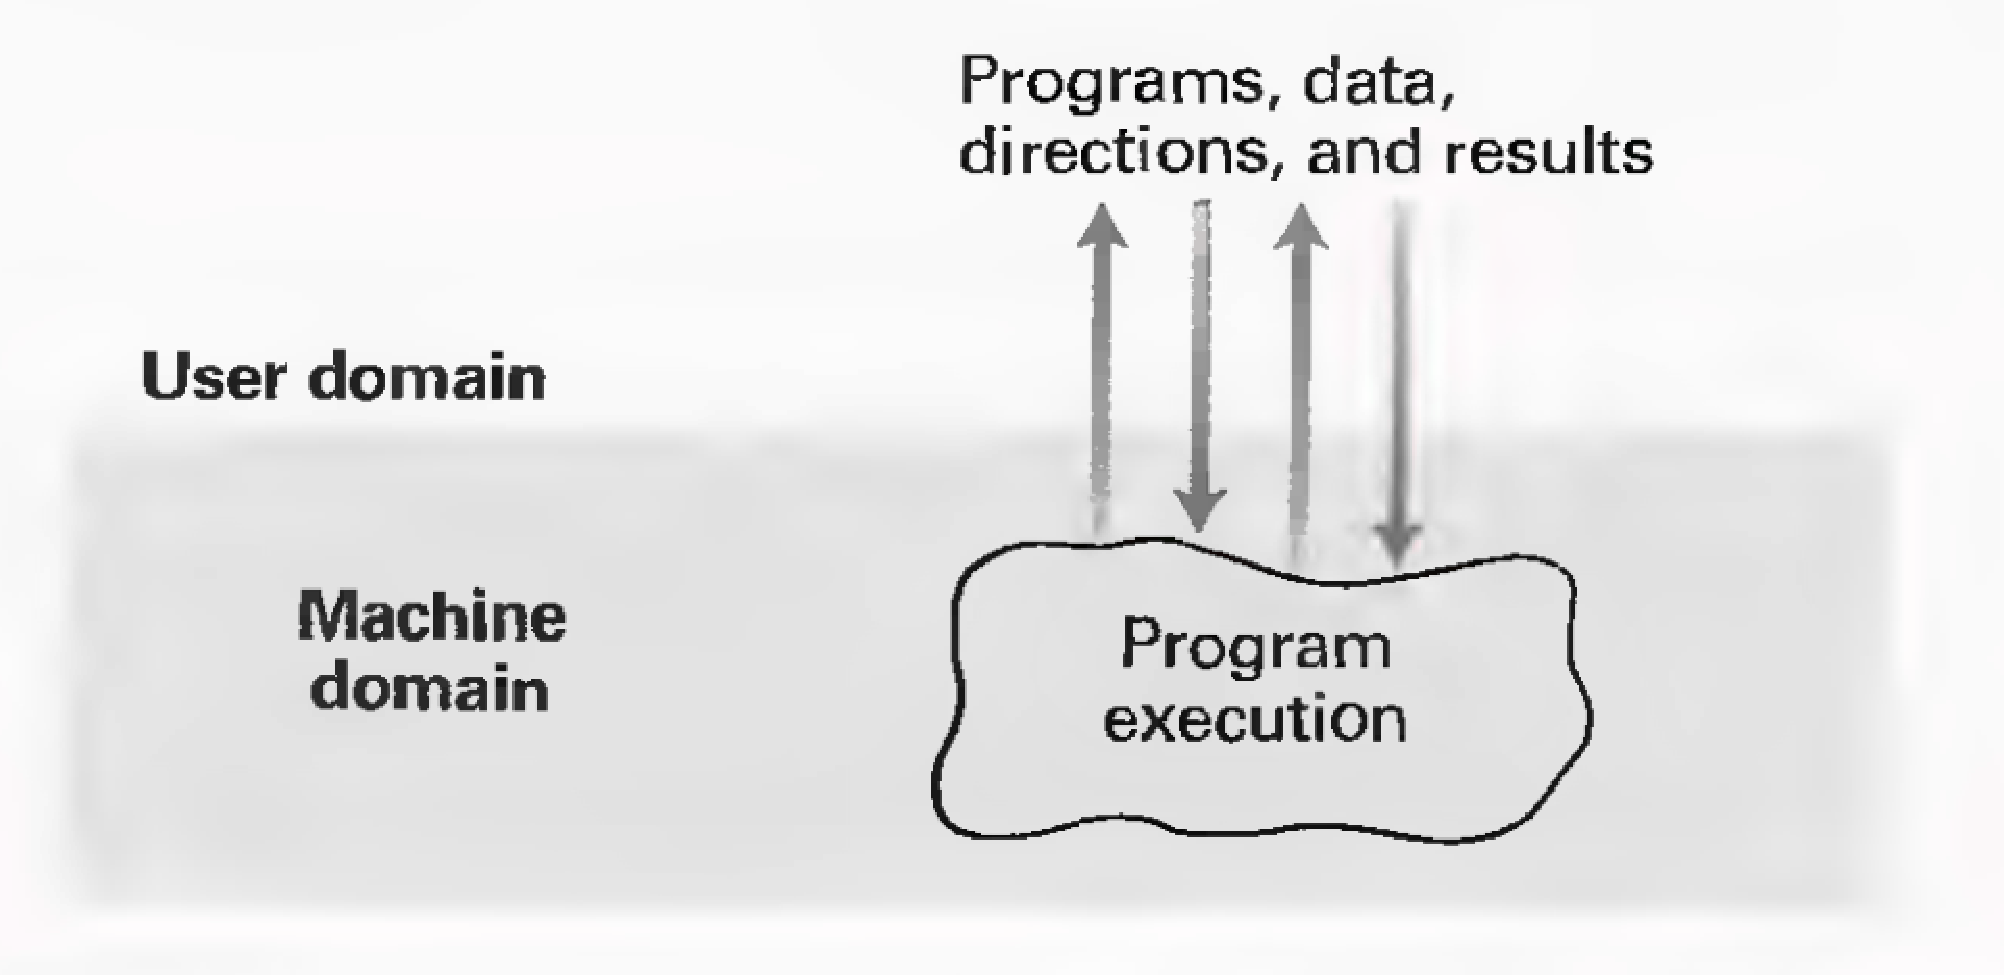
\includegraphics{ch4/fig32.pdf}}
\caption{Xử lý tương tác}
  \label{fig:fig3.2}
\end{figure}

Để việc xử lý tương tác thành công, điều hết sức quan trọng là các hoạt động của máy tính
phải đủ nhanh để phối hợp với các thao tác của người dùng thay vì ép người dùng phải chờ
đợi (ta có thể chờ đợi các các nhiệm vụ xử lý tiền lương thực hiện, nhưng không thể chấp
nhận nếu trong ứng dụng xử lý văn bản, máy tính không trả lời dấu nhắc lệnh khi các ký tự
được đánh). Các phục vụ của máy tính thoả mãn yêu cầu về thời gian được gọi là \textbf{xử
  lý thời gian thực}. Có nghĩa rằng, máy tính thực hiện nhiệm vụ đủ nhanh để để có thể
theo kịp các hoạt động của môi trường bên ngoài (thế giới thực).

Nếu hệ thống tương tác chỉ phục vụ một người dùng tại một thời điểm, vậy nó không gặp vấn
đề gì trong xử lý thời gian thực. Nhưng các máy tính trong những năm $1960$ và~$1970$ rất
đắt tiền, bởi vậy tại mỗi thời điểm, mỗi máy phải phục vụ rất nhiều người dùng. Họ làm
việc qua thiết bị đầu cuối ở xa để chuyển các phục vụ tương tác với máy, và vấn đề thời
gian thực trở thành một trở ngại. Nếu hệ điều hành cứ nhất định thực hiện một nhiệm vụ tại
một thời điểm, vậy thì chỉ một người dùng có thể thoả mãn phục vụ thời gian thực.

Một giải pháp cho vấn đề này là thiết kế hệ điều hành sao cho nó có thể chuyển việc thực
hiện các công việc khác nhau theo một chiến lược gọi là \textbf{chia sẻ thời gian thực},
đó là kỹ thuật chia thời gian thành các khoảng và sau đó hạn chế việc thực hiện mỗi công
việc trong một khoảng thời gian nhất định tại một thời điểm. Khi kết thúc mỗi khoảng, công
việc hiện hành bị đặt tạm ra bên ngoài và cho phép công việc khác tiếp tục thực hiện trong
khoảng tiếp theo. Bằng cách tráo đổi các công việc trước và sau một cách nhanh chóng theo
cách này, nó tạo ra cảm giác có nhiều công việc được chạy đồng thời. Phụ thuộc vào kiểu
công việc đang thực hiện, các hệ thống chia sẻ thời gian thực trước đây đã có thể cho phép
xử lý thời gian thực chấp nhận được với khoảng $30$ người sử dụng đồng thời. Ngày nay,
chia sẻ thời gian thực được sử dụng với hệ thống đơn người dùng cũng tốt như đa người
dùng, mặc dù về hình thức nó được gọi là \textbf{đa nhiệm}, để chỉ các hệ thống cho phép
(về mặt cảm giác) tại một thời điểm có thể có nhiều nhiệm vụ được thực hiện đồng thời.

Với sự phát triển của hệ điều hành đa người dùng và chia sẻ thời gian thực, một máy tính
đã được cấu hình như máy trung tâm kết nối với nhiều máy trạm. Từ các máy trạm này, người
dùng có thể giao tiếp trực tiếp với máy tính bên ngoài phòng máy thay vì phải gửi yêu cầu
tới người trực máy. Các chương trình sử dụng chung được lưu trữ trước trong thiết bị lưu
trữ khối của máy và hệ điều hành đã được thiết kế để thực hiện các chương trình này theo
yêu cầu từ các máy trạm. Vai trò người trực máy dần bị phai nhoà.

Ngày nay, về cơ bản không còn người trực máy nữa, đặc biệt trong lĩnh vực máy tính cá nhân
ở đó người sử dụng chịu mọi trách nhiệm thay người trực máy. Thậm chí hầu hết các máy tính
lớn không còn cần có người quản lý. Giờ đây công việc của người trực máy đã được thay bằng
người quản trị hệ thống, người chịu trách nhiệm quản lý hệ thống máy tính--có nhiệm vụ
theo dõi và thực hiện cài đặt thiết bị mới và phần mềm, bắt người dùng tôn trọng các quy
định như tạo tài khoản mới và thiết lập giới hạn không gian lưu trữ khối cho nhiều người
dùng, và cố gắng điều phối để giải quyết vấn đề gây ra trong hệ thống--hơn là thao tác với
máy trực tiếp bằng tay.

Tóm là, hệ điều hành đã phát triển từ một chương trình chỉ thực hiện nhiệm vụ đơn giản là
lưu trữ và thực hiện chương trình thành một hệ thống phức tạp điều phối việc chia sẻ thời
gian, bảo trì chương trình và các file dữ liệu trong các thiết bị lưu trữ khối của máy, và
trả lời trực tiếp yêu cầu từ người dùng.
 
Nhưng sự phát triển của các hệ điều hành vẫn chưa dừng ở đó. Sự phát triển của máy đa bộ
xử lý đã dẫn tới các hệ điều hành thực hiện đa nhiệm bằng cách gán các nhiệm vụ khác nhau
cho các bộ xử lý khác nhau thay vì chia sẻ thời gian của một bộ xử lý. Các hệ điều hành
này phải vật lộn với các vấn đề như \textbf{cân bằng tải} (các nhiệm vụ được gán một cách
động tới các bộ xử lý khác nhau sao cho mọi bộ xử lý được sử dụng một cách hiệu quả) cũng
như \textbf{scaling} (chia các nhiệm vụ thành các nhiệm vụ con tương thích với số bộ xử lý
có sẵn). Hơn nữa, sự phát triển của các mạng máy tính với nhiều máy ở khoảng cách xa được
kết nối với nhau đã dẫn tới tính cần thiết của phần mềm hệ thống để điều phối các hoạt
động của mạng. Bởi vậy lĩnh vực mạng (ta sẽ nghiên cứu chi tiết ở Chương \ref{} ) là một
trong nhiều chủ đề mở rộng của các hệ điều hành--mục đích là phát triển một hệ điều hành
đơn cho mạng rộng thay vì một mạng gồm nhiều hệ điều hành riêng lẻ.

\subsection*{Câu hỏi \& Bài tập}
\begin{enumerate}
\item Cho các ví dụ về hàng đợi. Trong mỗi trường hợp, chỉ ra tình
  huống vi phạm với cấu trúc FIFO.

\item Các hoạt động nào dưới đây yêu cầu xử lý thời gian thực?
  \begin{enumerate}
  \item In các nhãn thư điện tử

  \item Chơi một trò chơi trên máy tính

  \item Hiện các ký tự ra màn hình như chúng được nhập vào từ bàn phím

  \item Thực hiện chương trình dự báo tình trạng nền kinh tế trong năm
    tới
  \end{enumerate}

\item Nêu sự khác nhau giữa hệ điều hành xử lý thời gian thực và hệ
  điều hành tương tác?

\item Nêu sự khác nhau giữa hệ điều hành chia sẻ thời gian và đa nhiệm?
\end{enumerate}







%%% Local Variables: 
%%% mode: latex
%%% TeX-master: "../tindaicuong"
%%% End: 
